\documentclass{article}

% pacchetti 
\usepackage[italian]{babel}
\usepackage{graphicx}

% set images path 
\graphicspath{ {./images/} }
% specify different fonts for headings 


% pagina iniziale
\title{\textbf{\huge Design-Pattern}}

\author{Andrea Balbo Mossetto \\ Piaget Bouka \\ Davide Marietti \\ Edoardo Pastori}


% remove default print date in first page
\date{}
\begin{document}
	% sezione iniziale
	\maketitle
	
	\begin{center}
	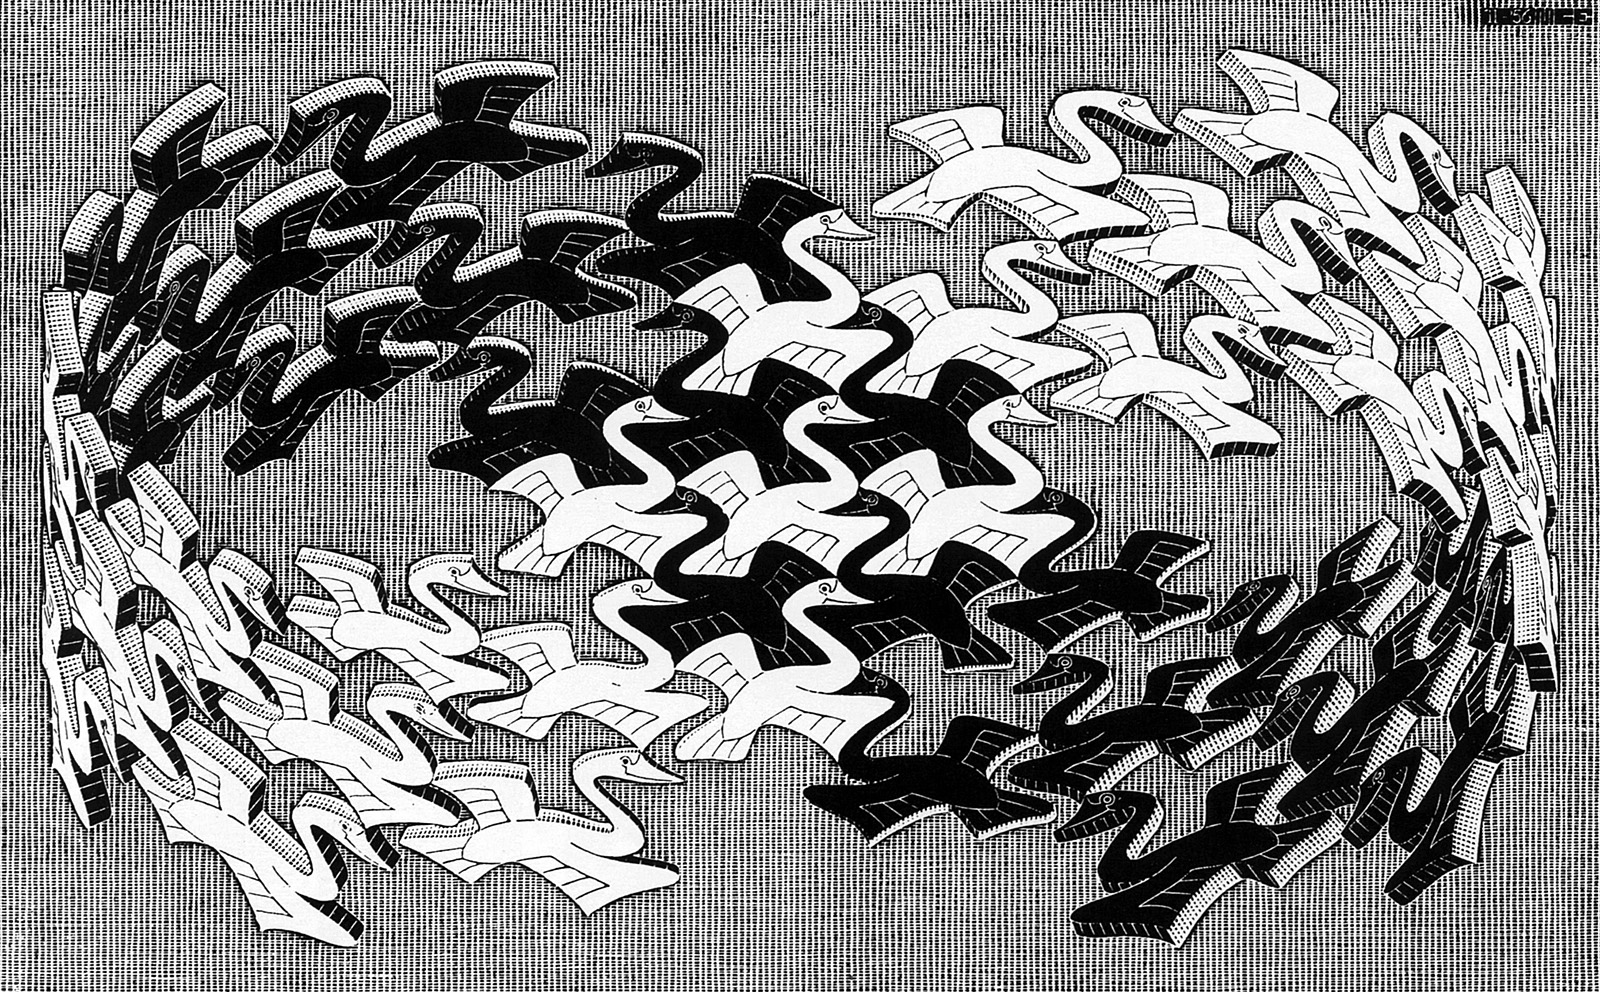
\includegraphics[scale=2]{design_pattern.jpeg}
	\end{center}
	
	
	\newpage
	
	\tableofcontents
	\newpage
	
	\listoffigures
	\newpage
	
	\abstract{}
	In questo documento \'e proposto il lavoro relativo alla realizzazione di un \textit{e-shop} di abbigliamento \textit{innovativo}. Una definizione pi\'u precisa di questo aggettivo ha richiesto una fase convergente, legata alla presa di coscienza delle caratteristiche proprie di quelli che sarebbero diventati i nostri \textit{competitors}, nonch\'e una fase divergente, attraverso la quale ci siamo soffermati sulle caratteristiche in linea con quella che iniziava a delinearsi con la nostra definizione di \textit{innovativo} mutuate da domini non appartenenti al mondo dell'\textit{e-shop} e dell'abbigliamento. 
	\\
	\\
	\textbf{TBC}
	
	\newpage
	
	% capitoli 
	\section{Elicitazione dei Requisiti}
	Questo capitolo raccoglie i requisiti che andranno poi analizzati, modellati e specificati nella fase di \textbf{Analisi dei Requisiti}. 
	\\
	\\
	I problemi comuni da evitare in questa fase iniziale, per uno sviluppo florido del progetto, riferiscono a 3 domini principali:
	\begin{enumerate}
		\item \textbf{Scopo}: i requisiti devono riflettere i bisogni del cliente
		\item \textbf{Comprensione}: \'e necessaria una buona comunicazione tra clienti, sviluppatori ed utenti per portare sul pratico i bisogni del cliente, che rifletteranno quelli degli utenti a cui vuole rivolgersi
		\item \textbf{Volatilit\'a}: i requisiti possono cambiare, non essere completi all'inizio dello sviluppo ed evolvere nel tempo; \'e quindi necessario definirli con quanta pi\'u perizia possibile in questa fase del processo
	\end{enumerate}
	
	Si rende quindi necessaria una stretta comunicazione con il cliente, rappresentato dalla Professoressa Bono, per giungere ad un insieme di conoscenze che permetta di superare i problemi esposti poco sopra. \\
	La strategia adottata \'e quella dell'\textbf{intervista}, alla quale siamo giunti dopo un \textit{brainstorming} che ci ha visto partecipi in un'iniziale definizione delle caratteristiche che, a nostro parere, dovrebbero appartenere ad un \textit{e-shop innovativo}.
	\\
	\\
	Le nostre riflessioni sono sintetizzate nella sezione successiva. 
	
	\subsection{Analisi di Mercato e Proposta di Prodotto} 
	
	\subsection{Intervista e Risultati}
	
	\newpage
	
	
	
	
	
\end{document}